%*******10********20********30********40********50********60********70********80
%% ----------------------------------------------------------------
%% Thesis.tex -- MAIN FILE (the one that you compile with LaTeX)
%% ---------------------------------------------------------------- 

%% This template is based on Graduate Thesis written by Sunil Patel,
% (ho based it on the ecsthesis template) under the LaTeX Project Public License.
% which can be found here: http://latex-project.org/lppl/
% in the hope that it will be easier to use and to scale down to your needs
% by Simon Ternsjö in 2013-10



% INSTRUCTIONS:

% The meaning is not to edit this document much, but to fill in information 
% in the different files in the folders;
% Settings, Frontpages, Chapters, Appendices and possibly Files,
% as well as the file Bibliography.bib

% This template is easy to scale down to suite your need, 
% simply comment the input statements explained below


% Set up the document:
\documentclass[a4paper, 11pt, oneside]{Thesis}  % Use the "Thesis" style, based on the ECS Thesis style by Steve Gunn

% Add more package in Package.tex:
% Add your own packages here, 
% these existing packages can be removed if necessary
% not that more packages are imported in Thesis.cls, '
%  but those should not be changed if you don't know what you are doing...


\usepackage[utf8]{inputenc} % for writing other that basic characters
\usepackage{graphicx}
\usepackage{caption}
\usepackage{subcaption}
\usepackage{multicol}
\usepackage[dvipsnames*,svgnames]{xcolor}
\usepackage{listings}
\usepackage{hyperref}
\usepackage{float}
\usepackage{bookmark}

\hypersetup{
    linkcolor=black,
    filecolor=magenta,      
    urlcolor=blue,
}


% Include any extra LaTeX packages required
\usepackage[square, numbers, comma, sort&compress]{natbib}  % Use the "Natbib" style for the references in the Bibliography
\usepackage{verbatim}  % Needed for the "comment" environment to make LaTeX comments
%5%\usepackage{vector}  % Allows "\bvec{}" and "\buvec{}" for "blackboard" style bold vectors in maths




% Use if you want:
%5%\graphicspath{Figures/}  % Location of the graphics files (set up for graphics to be in PDF format)
%5%\hypersetup{urlcolor=blue, colorlinks=true}  % Colours hyperlinks in blue, but this can be distracting if there are many links.

% Set your name, the title of the report and more in Administraitve.tex:
% This is where author, university, title and more is defined

% Personal information:
\newcommand{\myAuthorName}  {Andrea Spreafico}% Author Name
\newcommand{\myAuthorEmail} {asp005@post.uit.no} % Author email

\newcommand{\myTitle}       {INF-2900 Group Project - ScheduleIT} % Thesis title goes here
\newcommand{\mySubject}     {Computer Science} % Subject goes here
\newcommand{\myKeywords}    {ScheduleIT} % Keywords goes hear



% University information
\newcommand{\myUniversity}{University of Tromsø} %The Iniversity name goes here
\newcommand{\myUniversityWeb}{https://en.uit.no/startsida} %University Web Site URL Here (include http://
\newcommand{\myDepartment}{Department of Computer Science} % The Department goes here 
\newcommand{\myDepartmentWeb}{https://en.uit.no/om/enhet/forsiden?p_dimension_id=88138} % Department Web Site URL Here (include http://)
\newcommand{\myFaculty}{Faculty of Computer Science}
\newcommand{\myFacultyWeb}{https://uit.no/utdanning/program?p_document_id=279505}

%Degree, program or corse: ex: Master of Science, Engineering Physics
\newcommand{\myDegree}{Computer Science} % The degree, program or course-name goes here


% can be left untouched, both:
\newcommand{\myDate}{\today}
\newcommand{\myPartyalFulfillment}{A thesis submitted in partial fulfillment for the degree of Computer Science}

%% ----------------------------------------------------------------
\begin{document}
\frontmatter      % Begin Roman style (i, ii, iii, iv...) page numbering


% Here the first pages are imported, you can find them in the Frontpages folder
% Files in the subfolder Fixed does not need to be edited.
% If you don't need any of these sections, simply comment, or delete, the input-row\dfrac{•}{•}


%% All the pages before the chapters ------------------------------
% Set up the Title Page - DO NOT EDIT THIS, (if you don't want to ;)  )
% instead specify your name, title and more in "/Settings/Administrative.tex"
\title   {\myTitle}
\authors {Andrea Spreafico - asp005@post.uit.no \\
		  Stephan Abrahamsen - sab004@post.uit.no \\
		  Eva García Domingo - edo015@post.uit.no \\
		  Emil Nysted Hagen - eha092@post.uit.no\\
		  Siarhei Kulakou - sku019@post.uit.no
		  }
\addresses  {\groupname\deptname\\\univname}  
\date       {\myDate}
\subject    {\mySubject}
\keywords   {\myKeywords}
\date{29.05.17}

\maketitle
%% ----------------------------------------------------------------

\setstretch{1.3}  % It is better to have smaller font and larger line spacing than the other way round

% Define the page headers using the FancyHdr package and set up for one-sided printing
\fancyhead{}  % Clears all page headers and footers
\rhead{\thepage}  % Sets the right side header to show the page number
\lhead{}  % Clears the left side page header


\clearpage
\setstretch{1.3} % Reset the line-spacing to 1.3 for body text (if changed)
\pagestyle{fancy} % The page style headers have been "empty" all this time, 
                  % now use the "fancy" headers as defined before
\lhead{\emph{Contents}}  % Set the left side page header to "Contents"
\tableofcontents  % Write out the Table of Contents


%\setstretch{1.3} % Reset the line-spacing to 1.3 for body text (if changed)
\pagestyle{fancy} % The page style headers have been "empty" all this time, 
                  % now use the "fancy" headers as defined before
\lhead{\emph{List of Figures}}  % left side page header to "List if Figures"
\listoffigures  % Write out the List of Figures


%\clearpage  % Start a new page
\setstretch{1.3} % Reset the line-spacing to 1.3 for body text (if changed)
\pagestyle{fancy} % The page style headers have been "empty" all this time, 
                  % now use the "fancy" headers as defined before
\lhead{\emph{List of Tables}}  % left side page header to "List of Tables"
\listoftables  % Write out the List of Tables



%% The Body -------------------------------------------------------
\setstretch{1.3}  % Return the line spacing back to 1.3
\mainmatter	  % Begin normal, numeric (1,2,3...) page numbering
\pagestyle{fancy}  % Return the page headers back to the "fancy" style


% Include the chapters of the thesis, as separate files
% Just uncomment the lines as you write the chapters


%*******10********20********30********40********50********60********70********80

\chap{Introduction}


\section{Aim of the project}

Thinking of actual students' problems, we tried to find a solution to some of them. We have developed a whole  online platform for any group of people able to share a calendar. Our aim was to provide them with a tool that could organize  different schedules, being able to show each schedule separately or as a whole calendar that includes all the events.\\
Although our first target was students, the platform can be used by everyone who need an organizer. The only requirement a person needs is creating an account and he or she will be able to create a timetable and share it with people to join it.\\
People who join a timetable will be able to see the whole calendar but, obviously, they will not be able to edit it. by doing this, we have ensured the safety of a timetable.  In addition, in order to maintain the confidentiality of our users, the content of the website cannot be seen by someone without an account.\\
With the aim of helping new users to create accounts and to learn how to use the application, we have completely filled the Help and About pages. Furthermore, in case some question could not be answered through these pages, an email account has been created for contacting us.\\

\section{Aim of the course}
One of the purposes of this project was to learn how to work together in a cooperative environment. Some of the challenges we have successfully faced to are: sharing code, dealing with different schedules or finding a common idea of what to do and how to do it. We have learnt that having a meeting once per week is unavoidable for sharing ideas, problems and struggles, asking for help and being updated.\\
Finally, another important objective consisted on learning to use the framework Ruby on Rails. We found that it is such a powerful web developer, hard to use for the first time, but very sensitive to any change. That is, with so few code lines you can make big changes in your application. In addition, compared with others frameworks, it is quite easy to put together the logic with the graphics: Ruby helps you as much as a software can. % Introduction

%*******10********20********30********40********50********60********70********80
\chap{Background Theory}
    
\section{Agile Software Development} \label{Agile}
\vspace{-5mm}
Agile is an umbrella term for methods of software development, based on the idea of developing software incrementally, instead of all at once. The project itself is broken down into several \textit{user stories}, where each story gets a weighted value based on difficulty. The stories are divided into short cycles called \textit{iterations}.\cite{agile:nutshell}

\subsection{User stories}
\vspace{-5mm}
User stories are very high-level definitions of project requirements, and contain just enough information so the developers can estimate a time frame for completing it. The usual format of a user story looks somewhat like this:
\vspace{-5mm}
\begin{center}
	\textit{As a (role) I want (something) so that (benefit).}
\end{center}
\vspace{-5mm}
Each story is expected to yield a contribution to the overall completion if the product.\cite{agile:modeling}

\pagebreak
\subsection{Iterations}\label{iter}\vspace{-5mm}
An iteration is a short period of time where some of the user stories are implemented completely. This means that for each iteration a new part of the project is fully implemented and tested. Each iteration usually consists of different renditions of these parts: plan, design, build, test, and review. 
\begin{figure}[H]
	\centering
	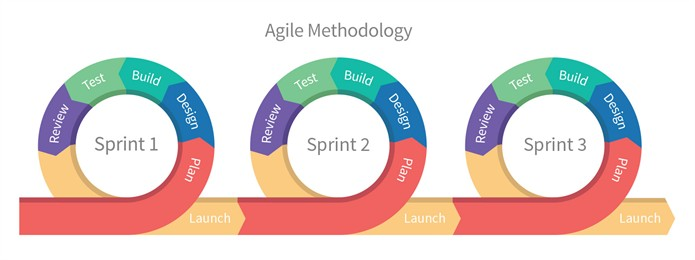
\includegraphics[trim={0 0 0 0},clip,width=0.8\textwidth]{Files/agile.jpg}
	\caption{Visualization of the iterations\cite{agile:figure}.}
	\label{fig: MVC}
\end{figure}

\subsection{Agile vs. Waterfall}
Another software development method is Waterfall, which is a more linear, straight-forward approach than Agile. The different stages of Waterfall differ, depending on who the developers are, but usually looks something like this\cite{w-vs-a}:
\vspace{-5mm}
\begin{itemize}\setlength{\itemsep}{-5pt}
	\item[1.] Establish requirements.
	\item[2.] Design.
	\item[3.] System testing.
	\item[4.] User acceptance testing.
	\item[5.] Fix issues.
	\item[6.] Delivery
\end{itemize}
In the Waterfall approach each of these elements are separate stages, and you can't start a new stage until the previous one is completed. A Waterfall project's requirements are usually defined in advance, and previous stages are off limits once completed, meaning you can't go back and change an already completed stage.\\\\
Agile, on the other hand is far more flexible, and allows you to move freely through the project as desired. The requirements are expected to change and expand during the course of the project. Agile is also far more forgiving when it comes to changing previously implemented features.\\
Waterfall and Agile are not very similar in regards to the development process, yet they both share the same end-goal; delivering the product efficiently.\cite{smartsheet}

\section{Ruby on Rails} 
\vspace{-5mm}
Ruby on Rails (RoR) is a server-side web application framework. RoR is a model–view–controller framework, providing default structures for a database, a web service, and web pages.\cite{wiki:RoR}

\begin{figure}[H]
	\centering
    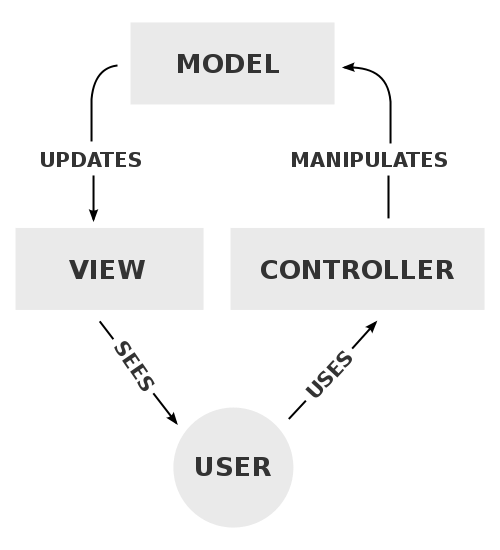
\includegraphics[trim={0 0 0 0},clip,width=0.4\textwidth]{Files/MVC.png}
    \caption{Diagram of interactions within the MVC pattern.\cite{wiki:mvc} }
    \label{fig: MVC}
\end{figure}
\vspace{-3mm}

\textbf{The Model} contains the data and the state if the application, and it has no knowledge of the user interface, so it can be reused.\\
\textbf{The View} generates the user interface which presents the user with the data, but isn't able to do any processing. Different views are able to access the same model for different usages.\\
\textbf{The Controller} interacts with the outside world through the views, interacts with the model, and displays the appropriate view to the user.




 % Background Theory 

%*******10********20********30********40********50********60********70********80
\chap{Analysis and Design}
Concentrate on explaining the decisions made and the reasons for them.
\section{Web application architecture}

\section{Models design}

\begin{figure}[H]
	\centering
    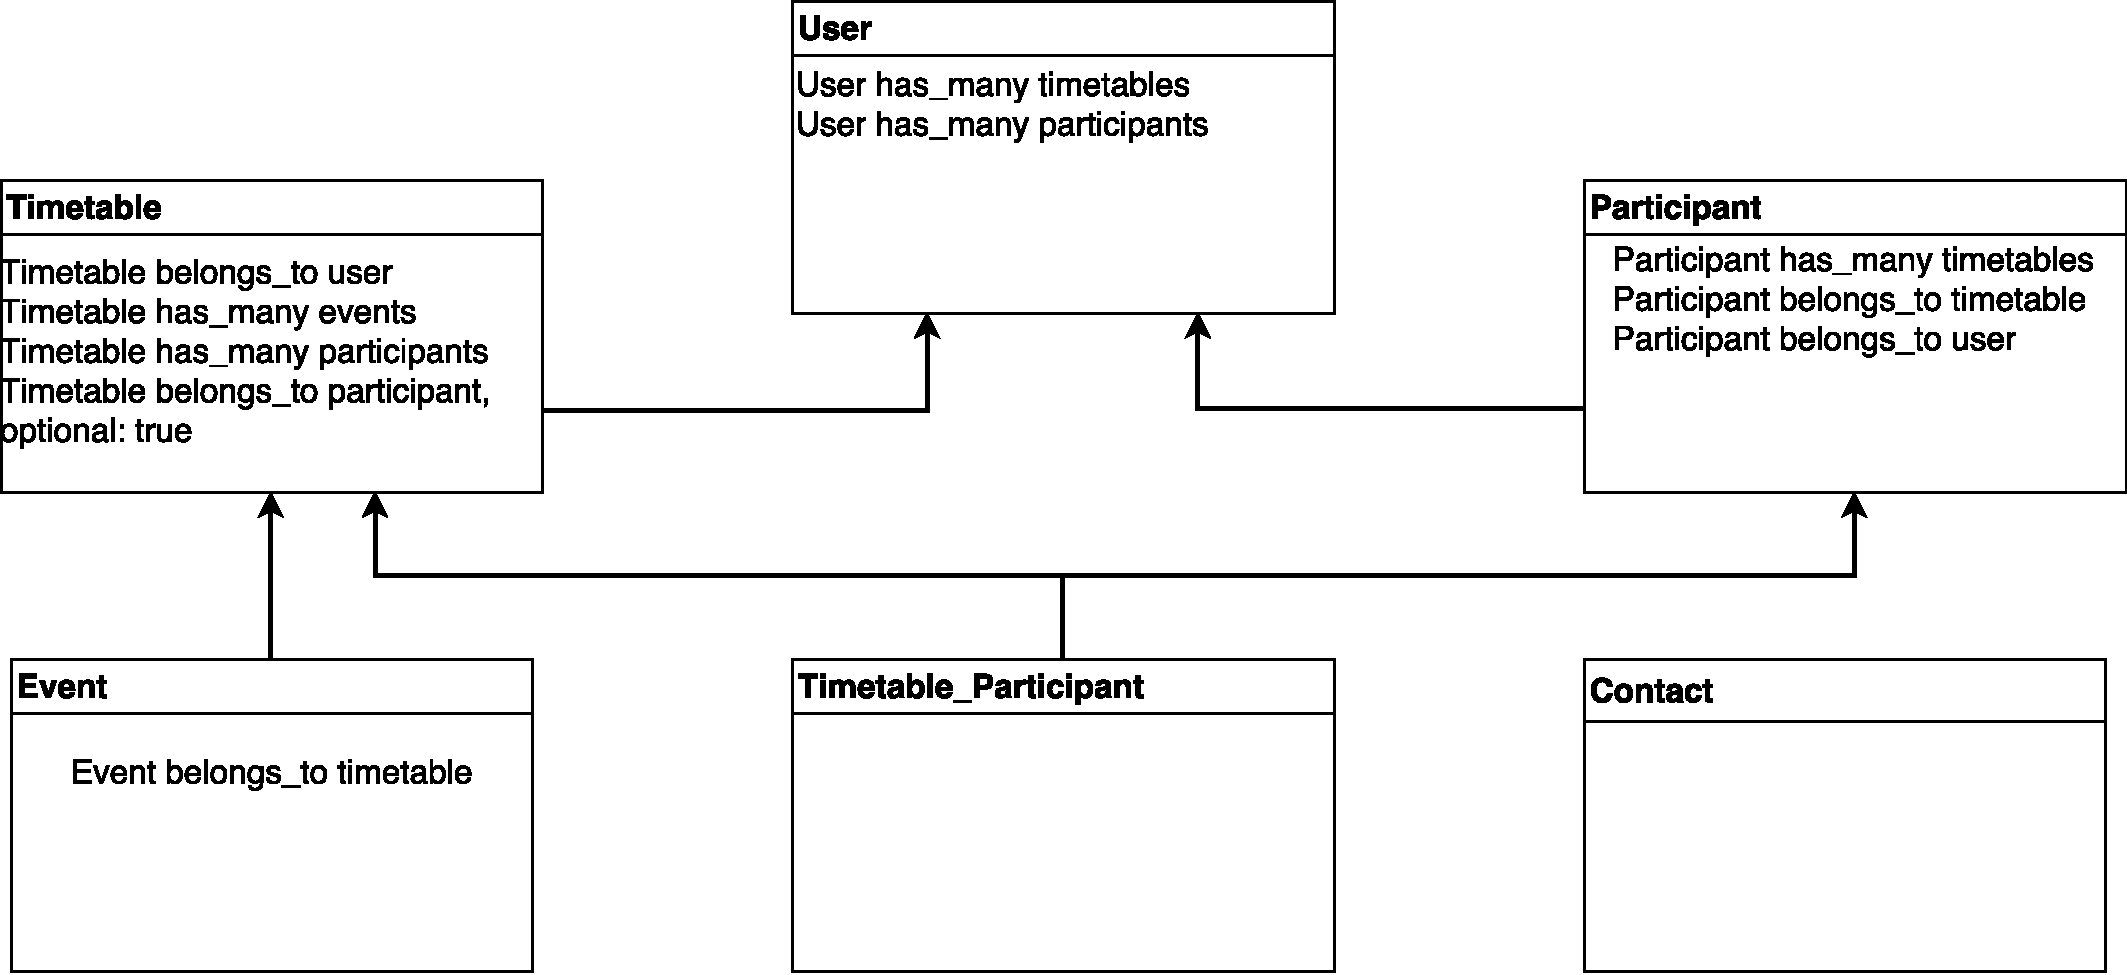
\includegraphics[trim={0 0 0 0},clip,width=1\textwidth]{Files/Models.pdf}
    \caption{Implemented models.}
    \label{fig: Models}
\end{figure}

\subsection{User}
The user model is responsible for keeping track of the application's user information. It is directly related to the timetable and participant models, because each user must be able to own several timetables, as well as participating.\\ 
The rest of the model is set up to ensure that the user information is correct. It validates the user e-mail, uses a Bcrypt function to ensure that all users have passwords, and in turn, hashes the password string so that no plaintext passwords are stored in the database. An added feature also allows the user to upload an avatar (profile picture) for their profile. 

\subsection{Session}
\subsection{Timetable}
The timetable
\subsection{Event}
\subsection{Participant}
The participant model was the last one on implementation, and the most difficult, due to the fact it has relations with two other models:
\begin{itemize} \setlength{\itemsep}{-5pt}
\item Users: a participant is a user. That is, one-to-many relationship.
\item Timetables: many-to-many relationship
\begin{itemize} \setlength{\itemsep}{-5pt}
\item A participant "belongs" to a timetable, but can participate in many timetables.
\item A timetable can have many participants.
\end{itemize}
\end{itemize} 
Obviously, the fields for the foreign keys to user and timetable can not be empty.\\
The many-to-many relation was done separating the "belongs\_to/has\_many" instead using the formula "has\_and\_belongs\_to\_many" because this last one caused us problems in the admin page and when trying to use the foreign keys. These problems were caused  because the use of the foreign key as \textit{user.participant} were not different from \textit{user.participants} (there were not two different relationships).
\subsection{Contact}
The contact model is a small and simple one, but it contains the necessary parts for a proper e-mail header. 
Whenever a user submits a new contact form, the model validates the fields of the form, as well as one "invisible" field, 
used for catching spam bots. This "spam catcher" works by refusing to submit forms where the field \textit{nickname} 
contains any characters. Since the field being hidden by some CSS code, we know that a human can't see this field, unless they have access to the code, in which case it's most likely a robot of some kind.
 
 % Analysis and Design

\chap{Implementation}
 % Team Work

\chap{Discussion}
It is possible to say that the results obtaiend are achieving most of the initil goals of this project. 
Like reported in the introduction part [\ref{Introduction}], the two main goals of this work were: 
\vspace{-10mm}
\begin{itemize}
 \setlength{\itemsep}{-5pt}
 \item Implement a web application that provides a scheduler.
 \item Apply the development agile process.s
\end{itemize}

The resulting web application actually provides a online scheduler that contains several utilities and functions. Almost all the user stories that were supposed to be realized have been correctly implemented during this work. In particular, the results provide an answer to the initial goals of the scheduler implementation. 

Further more, during the whole development process the agile approach had a high consideration and priorization from all the members of the team. Has been actually possible to see a big improvement about the agile process application between the beginning and the end of this work.

More details about evaluation and limitations of the implemented project can be find in the next section.
\section{Evaluation and Limitations}
\label{Evaluation}
The following list reports the main limitations that have been found during the implementation process.
\vspace{-5mm}
\begin{itemize}
 \setlength{\itemsep}{-5pt}
\item Time limitation has probably been the biggest issue. Working on a project with several people means that you have to somehow find a way to combine different schedules, that is not always that easy. Also a quite short project deadline implies a limitated extra features implementation.
\item Limitated amount of previous knowledges and experiences about both Ruby on Rails and agile process imply that each single member of the team, mainly during the first part of the work, had to document himself about it. It means a significant investment of time and effort focused about get knowledge and less about web application's extra features. 
\end{itemize}

Despite of the limitations that have been reported above here, this work provided to all the team member:
\vspace{-5mm}
\begin{itemize}
 \setlength{\itemsep}{-5pt}
\item New knowledges and experiences about agile process, in particular how to handle a group project, communication and collaboration with other people.
\item Improved abilities about gitlab/github usage, since it has been an indispensable instrument during the whole work.
\item Fist but really complete approach with framework Ruby on Rails.
\end{itemize}



\section{Team efforts and Time lists}
One of the most important thing during the whole development process was splitting the jobs between the team members in a efficient way and at the same time let every single team member put the same effort into the project.\\
Was actually asked to every single team member to constantly contribute at the work as much as possible. How it's possible to see in the following graphic, there has been a quite constant effort and work on the project.
\begin{figure}[H]
	\centering
    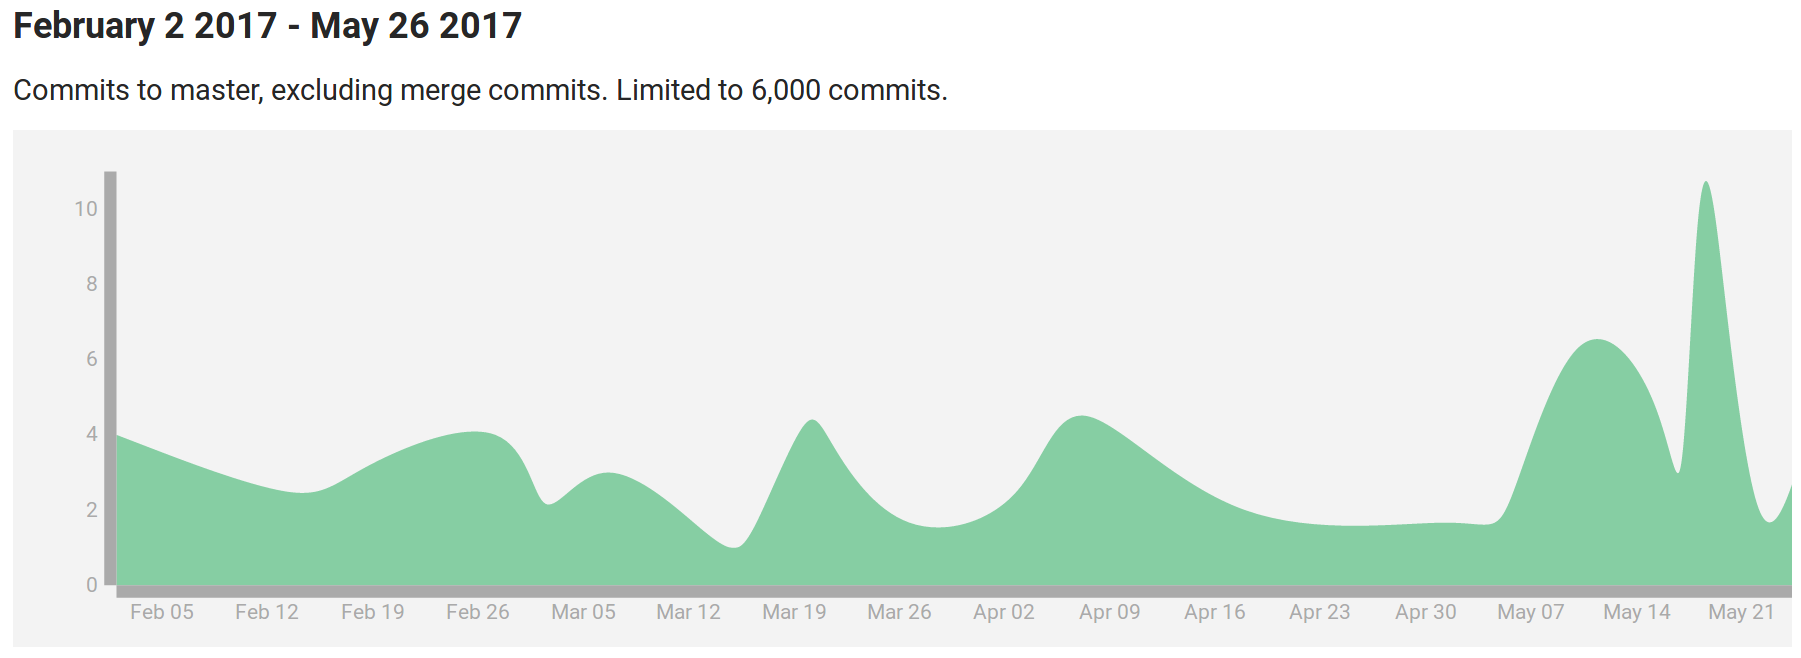
\includegraphics[trim={0 0 0 0},clip,width=1\textwidth]{Files/commitsToMaster.png}
    \caption{Commits to master, excluding merge commits.\\ \textbf{Source:} https://inf2900v17.cs.uit.no/team1/coffee-overflow/graphs/master}
    \label{fig: MVC}
\end{figure}


 % Discussion

\chap{Conclusions}

\section{Summary}
What have you achieved?

\section{Further Works on the project}
\vspace{-5mm}
\begin{itemize}
 \setlength{\itemsep}{-5pt}
\item \textbf{Develop the web application like a smartphone application}

\item \textbf{Public/Private schedules}\\
- Send participation requests.\\
- Ask to join

\item \textbf{Possibility of comment events}

\item \textbf{Possibility to follow a single event instead of the whole timetable}
\end{itemize}

\section{Further Works on the team work process}
\vspace{-5mm}
\begin{itemize}
 \setlength{\itemsep}{-5pt}
 \item
 \item
\end{itemize} % Conclusions, Evaluation and further work

\chapter{Bibliography}
 % Bibliography


%% Appendices -----------------------------------------------------
\addtocontents{toc}{\vspace{2em}} % Add a gap in the Contents, for aesthetics
\lhead{\emph{Appendices}}  % Change the left side page header to "Appendices"
\appendix % Cue to tell LaTeX that the following 'chapters' are Appendices

%\chap{An Appendix} % Appendix Title

%\input{Appendices/AppendixB} % Appendix Title

%\input{Appendices/AppendixC} % Appendix Title

\end{document}  % The End
%% ----------------------------------------------------------------